\begin{figure}[ht]
  \centering
  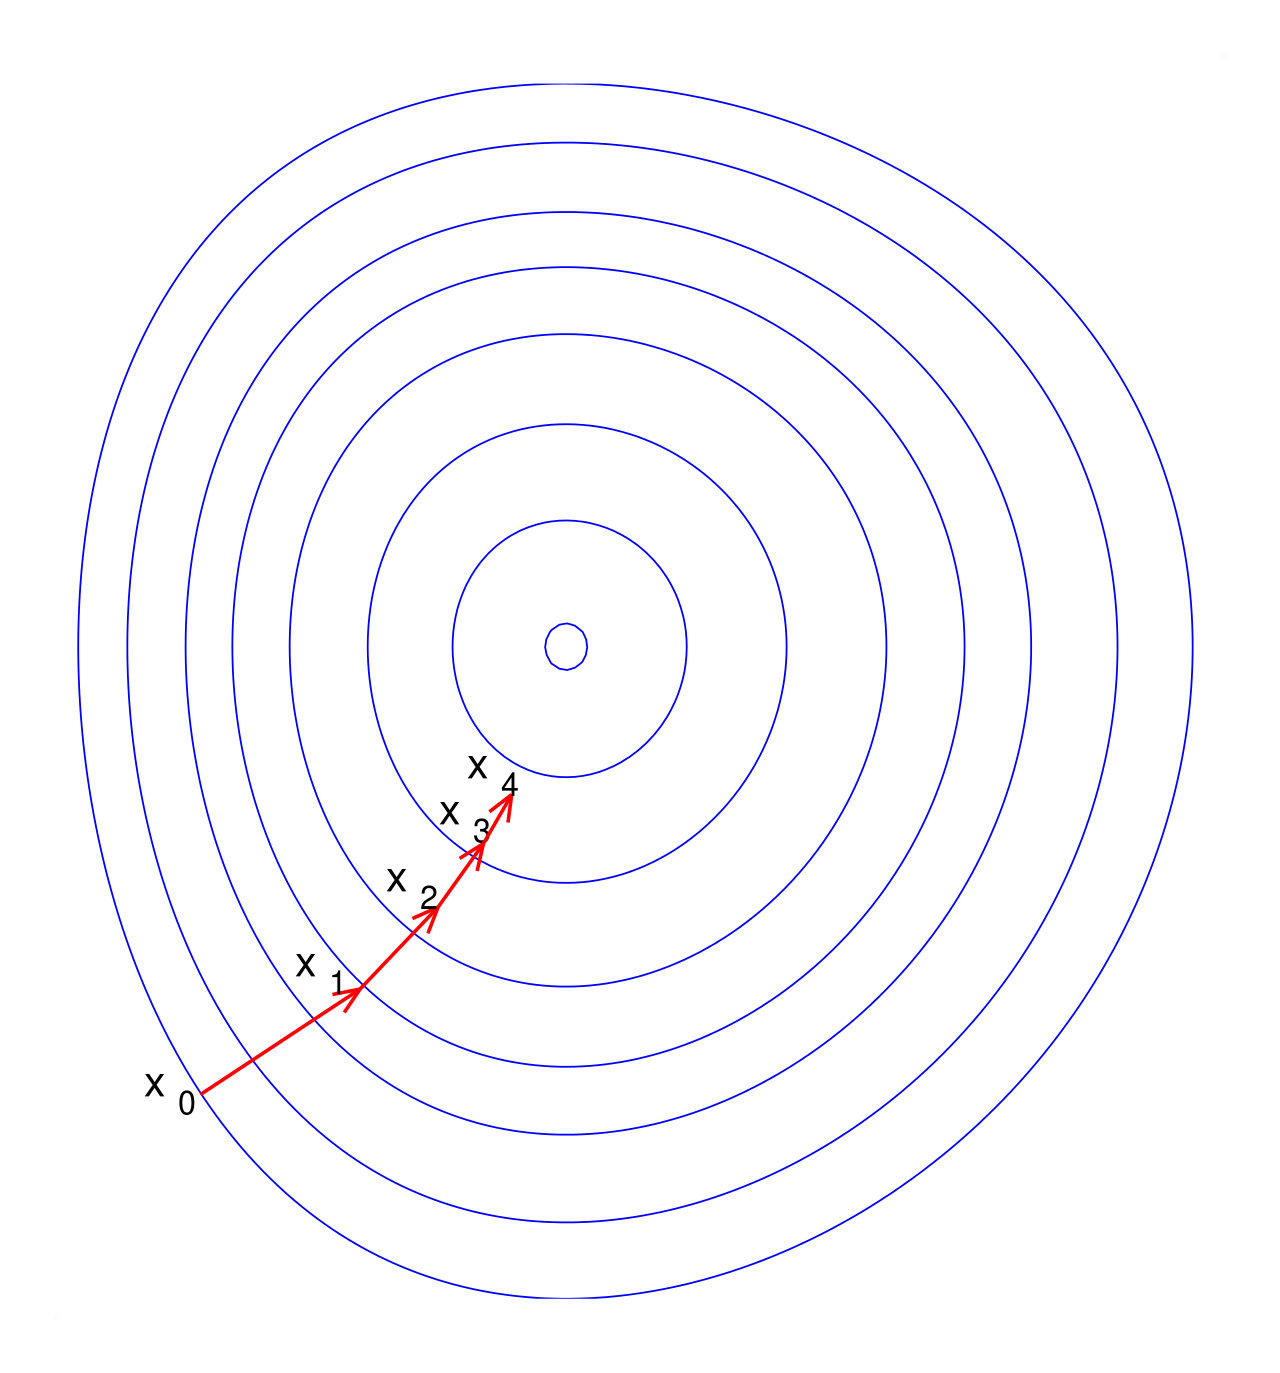
\includegraphics[width=.6\textwidth]{gradient-descent}
  \caption[An illustration of gradient descent.]{An illustration of the gradient
    descent algorithm. The blue lines represent level sets of a function, sets
    of points that have the same gradient. The $x$'s represent where in the
    range of the function the output calculated with the weights at the
    current step is. Five steps are shown, numbered 0--4.}
  \label{fig:grad-desc}
\end{figure}
  